% presentation
\documentclass{beamer}
\usetheme[height=7mm]{Rochester}
\usecolortheme{rose}

% handout

%\documentclass[handout]{beamer}
%\usepackage{pgfpages} \pgfpagesuselayout{8 on 1}[a4paper]

%\documentclass[mathserif]{article}
%\usepackage{beamerarticle}

\usepackage{amsmath}
\usepackage{comment}
\usepackage{amssymb,amsfonts}
\usepackage[T1]{fontenc}
\usepackage{lmodern}
\usepackage{tikz}
%\usepackage{simpsons}
\usepackage{marvosym}
\usepackage{color}
\usepackage{multirow}
\usepackage{pgffor}
\usepackage{pgfplots}
\usepackage[slide,algoruled,titlenumbered,vlined,noend,linesnumbered,]{algorithm2e}

\usefonttheme{structurebold}

\setbeamertemplate{footline}[frame number]
\setbeamertemplate{navigation symbols}{}
\setbeamerfont{smallverb}{size*={73}}
\usefonttheme[onlymath]{serif}
\setbeamertemplate{theorems}[numbered]
\newtheorem{construction}[theorem]{Construction}
\newtheorem{proposition}[theorem]{Proposition}

\AtBeginSection[] {
  \begin{frame}
    \frametitle{Content}
    \tableofcontents[currentsection]
  \end{frame}
  \addtocounter{framenumber}{-1}
}

\usetikzlibrary[shapes.arrows]
\usetikzlibrary{shapes.geometric}
\usetikzlibrary{backgrounds}
\usetikzlibrary{positioning}
\usetikzlibrary{calc}
\usetikzlibrary{intersections}
\usetikzlibrary{fadings}
\usetikzlibrary{decorations.footprints}
\usetikzlibrary{patterns}
\usetikzlibrary{shapes.callouts}
\usetikzlibrary{fit}
%handout

\providecommand{\abs}[1]{\lvert#1\rvert}

\tikzset{every picture/.style={line width=1pt,show background rectangle},background rectangle/.style={fill=blue!10,rounded corners=2ex}}

\newcommand{\Bob}[3]{ \begin{scope}[shift={(#1,#2)},scale=#3]
  \draw (0,0) circle (0.95 and 1);
  \fill (-0.3,-0.1) circle (0.1);
  \fill (+0.3,-0.1) circle (0.1);
  \draw (0.35,-0.5) arc (-70:-110: 1 and 0.4);
  \draw (-0.3,0.5) arc (-10:-80: 0.8 and 0.8);
  \draw (-0.5,0.8) arc (190:255: 2 and 1);
  \draw (-0.7,0.9) -- +(0.2,-0.09) -- +(0.25,0.2);
  \end{scope} }

\newcommand{\Alice}[3]{ \begin{scope}[shift={(#1,#2)},scale=#3]
  \draw (0,0) circle (0.95 and 1);
  \fill (-0.3,-0.1) circle (0.1);
  \fill (+0.3,-0.1) circle (0.1);
  \draw (0.35,-0.5) arc (-70:-110: 1 and 0.4);
  \draw (0.3,1.3) arc (20:-100: 1.4 and 1);
  \draw (0.5,1.3) arc (150:260: 1 and 1);
  \draw (0.41,1.3) circle (0.35);
  \end{scope} }

  \newcommand{\Evil}[3]{ \begin{scope}[shift={(#1,#2)},scale=#3]
    \draw (0,0) circle (0.95 and 1);
    \fill (-0.1,-0.1) -- +(-0.2,-0.1) -- +(-0.4,0.2); %eye
    \fill (0.1,-0.1) -- +(0.2,-0.1) -- +(0.4,0.2);
    \draw (0.35,-0.5) arc (-70:-110: 1 and 0.4);
    %\fill (0.3,-0.5) -- +(-0.1,-0.2) -- +(-0.2,-0.02);
    %\fill (-0.3,-0.5) -- +(0.1,-0.2) -- +(0.2,-0.02);
    \fill (0.3,0.7) -- +(0.5,0.4) -- +(0.4,-0.2); % horn
    \fill (-0.3,0.7) -- +(-0.5,0.4) -- +(-0.4,-0.2);
    %\draw (0.3,1.3) arc (20:-100: 1.4 and 1);
    %\draw (0.5,1.3) arc (150:260: 1 and 1);
    %\draw (0.41,1.3) circle (0.35);
    \end{scope} }

\newcommand{\Charlie}[3]{ \begin{scope}[shift={(#1,#2)},scale=#3]
    \draw (0,0) circle (0.95 and 1);
    \filldraw[fill=black!20] (-0.35,-0.1) circle (0.25);
    \filldraw[fill=black!20] (+0.35,-0.1) circle (0.25);
    %\draw (0.9,0.2) to [bend left] (-0.9,0.2);
    \draw (0.2,0) to [bend left] (-0.2,0);


    %\draw (0.3,0.7) to [bend right] (-0.3,0.7);
    %\draw (0.4,0.5) to [bend right] (-0.4,0.5);
    %\draw (0.35,-0.5) arc (-70:-110: 1 and 0.4);
    \draw (-0.7,-0.6) to [bend right] (0,-0.6) to [bend right] (0.7,-0.6) to [bend right]  (0,-0.5)  to [bend right]  cycle ;
    %\draw (0.3,1.3) arc (20:-100: 1.4 and 1);
    %\draw (0.5,1.3) arc (150:260: 1 and 1);
    %\draw (0.41,1.3) circle (0.35);
    \end{scope} }

\author{Yu Zhang}
\institute{Harbin Institute of Technology}
\date[Crypto'22A]{Cryptography, Autumn, 2022}

%% presentation
\documentclass{beamer}
\usetheme[height=7mm]{Rochester}
\usecolortheme{rose}

% handout

%\documentclass[handout]{beamer}
%\usepackage{pgfpages} \pgfpagesuselayout{8 on 1}[a4paper]

%\documentclass[mathserif]{article}
%\usepackage{beamerarticle}

\usepackage{amsmath}
\usepackage{comment}
\usepackage{amssymb,amsfonts}
\usepackage[T1]{fontenc}
\usepackage{lmodern}
\usepackage{tikz}
%\usepackage{simpsons}
\usepackage{marvosym}
\usepackage{color}
\usepackage{multirow}
\usepackage{pgffor}
\usepackage{pgfplots}
\usepackage[slide,algoruled,titlenumbered,vlined,noend,linesnumbered,]{algorithm2e}

\usefonttheme{structurebold}

\setbeamertemplate{footline}[frame number]
\setbeamertemplate{navigation symbols}{}
\setbeamerfont{smallverb}{size*={73}}
\usefonttheme[onlymath]{serif}
\setbeamertemplate{theorems}[numbered]
\newtheorem{construction}[theorem]{Construction}
\newtheorem{proposition}[theorem]{Proposition}

\AtBeginSection[] {
  \begin{frame}
    \frametitle{Content}
    \tableofcontents[currentsection]
  \end{frame}
  \addtocounter{framenumber}{-1}
}

\usetikzlibrary[shapes.arrows]
\usetikzlibrary{shapes.geometric}
\usetikzlibrary{backgrounds}
\usetikzlibrary{positioning}
\usetikzlibrary{calc}
\usetikzlibrary{intersections}
\usetikzlibrary{fadings}
\usetikzlibrary{decorations.footprints}
\usetikzlibrary{patterns}
\usetikzlibrary{shapes.callouts}
\usetikzlibrary{fit}
%handout

\providecommand{\abs}[1]{\lvert#1\rvert}

\tikzset{every picture/.style={line width=1pt,show background rectangle},background rectangle/.style={fill=blue!10,rounded corners=2ex}}

\newcommand{\Bob}[3]{ \begin{scope}[shift={(#1,#2)},scale=#3]
  \draw (0,0) circle (0.95 and 1);
  \fill (-0.3,-0.1) circle (0.1);
  \fill (+0.3,-0.1) circle (0.1);
  \draw (0.35,-0.5) arc (-70:-110: 1 and 0.4);
  \draw (-0.3,0.5) arc (-10:-80: 0.8 and 0.8);
  \draw (-0.5,0.8) arc (190:255: 2 and 1);
  \draw (-0.7,0.9) -- +(0.2,-0.09) -- +(0.25,0.2);
  \end{scope} }

\newcommand{\Alice}[3]{ \begin{scope}[shift={(#1,#2)},scale=#3]
  \draw (0,0) circle (0.95 and 1);
  \fill (-0.3,-0.1) circle (0.1);
  \fill (+0.3,-0.1) circle (0.1);
  \draw (0.35,-0.5) arc (-70:-110: 1 and 0.4);
  \draw (0.3,1.3) arc (20:-100: 1.4 and 1);
  \draw (0.5,1.3) arc (150:260: 1 and 1);
  \draw (0.41,1.3) circle (0.35);
  \end{scope} }

  \newcommand{\Evil}[3]{ \begin{scope}[shift={(#1,#2)},scale=#3]
    \draw (0,0) circle (0.95 and 1);
    \fill (-0.1,-0.1) -- +(-0.2,-0.1) -- +(-0.4,0.2); %eye
    \fill (0.1,-0.1) -- +(0.2,-0.1) -- +(0.4,0.2);
    \draw (0.35,-0.5) arc (-70:-110: 1 and 0.4);
    %\fill (0.3,-0.5) -- +(-0.1,-0.2) -- +(-0.2,-0.02);
    %\fill (-0.3,-0.5) -- +(0.1,-0.2) -- +(0.2,-0.02);
    \fill (0.3,0.7) -- +(0.5,0.4) -- +(0.4,-0.2); % horn
    \fill (-0.3,0.7) -- +(-0.5,0.4) -- +(-0.4,-0.2);
    %\draw (0.3,1.3) arc (20:-100: 1.4 and 1);
    %\draw (0.5,1.3) arc (150:260: 1 and 1);
    %\draw (0.41,1.3) circle (0.35);
    \end{scope} }

\newcommand{\Charlie}[3]{ \begin{scope}[shift={(#1,#2)},scale=#3]
    \draw (0,0) circle (0.95 and 1);
    \filldraw[fill=black!20] (-0.35,-0.1) circle (0.25);
    \filldraw[fill=black!20] (+0.35,-0.1) circle (0.25);
    %\draw (0.9,0.2) to [bend left] (-0.9,0.2);
    \draw (0.2,0) to [bend left] (-0.2,0);


    %\draw (0.3,0.7) to [bend right] (-0.3,0.7);
    %\draw (0.4,0.5) to [bend right] (-0.4,0.5);
    %\draw (0.35,-0.5) arc (-70:-110: 1 and 0.4);
    \draw (-0.7,-0.6) to [bend right] (0,-0.6) to [bend right] (0.7,-0.6) to [bend right]  (0,-0.5)  to [bend right]  cycle ;
    %\draw (0.3,1.3) arc (20:-100: 1.4 and 1);
    %\draw (0.5,1.3) arc (150:260: 1 and 1);
    %\draw (0.41,1.3) circle (0.35);
    \end{scope} }

\author{Yu Zhang}
\institute{Harbin Institute of Technology}
\date[Crypto'22A]{Cryptography, Autumn, 2022}

%\input{1introduction.tex}
%\input{2perfectlysecret.tex}
%\input{3privatekey.tex}


\title{Introduction}

\begin{document}
\maketitle
\begin{frame}
\frametitle{Outline}
\tableofcontents
\end{frame}
\section{Cryptography and Modern Cryptography}
\begin{frame}\frametitle{What is Cryptography?}
\begin{itemize}
\item \textbf{Cryptography}: from Greek \emph{krypt\'os}, ``hidden, secret''; and \emph{gr\'{a}phin}, ``writing''
\item \textbf{Cryptography}: the art of writing or solving codes.\\ (Concise oxford dictionary 2006)
\item \textbf{Codes}: a system of prearranged signals, especially used to ensure secrecy in transmitting messages. \\ (\emph{code word} in cryptography)
\item \textbf{1980s}: from Classic to Modern; from Military to Everyone
\item \textbf{Modern cryptography}: the scientific study of mathematical techniques for securing digital information, systems, and distributed computations against adversarial attacks
\end{itemize}
\end{frame}
\begin{frame}\frametitle{What is cryptography? [xkcd:504]}
\begin{figure}
\begin{center}
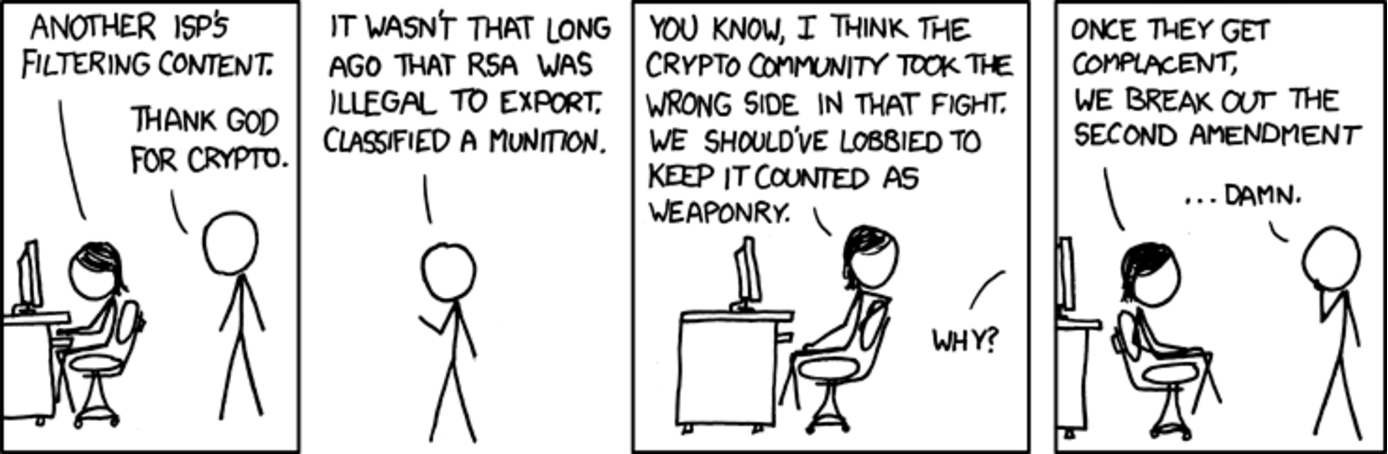
\includegraphics[width=100mm]{pic/legal} 
\end{center}
\end{figure}
\end{frame}
\section{The Setting of Private-Key Encryption}
\begin{frame}\frametitle{Private-Key Encryption}
\begin{itemize}
\item \textbf{Goal}: to construct \textbf{ciphers} (encryption schemes) for providing secret communication between two parties sharing \textbf{private-key} (the symmetric-key) in advance
\item \textbf{Implicit assumption}: there is some way of initially sharing a key in a secret manner
\item \textbf{Disk encryption}: the same user at different points in time
\end{itemize}
\end{frame}
\begin{frame}\frametitle{Alice, Bob  [xkcd:1323]}
Changing the names would be easier, but if you're not comfortable lying, try only making friends with people named Alice, Bob, Carol, etc.
\begin{figure}
\begin{center}
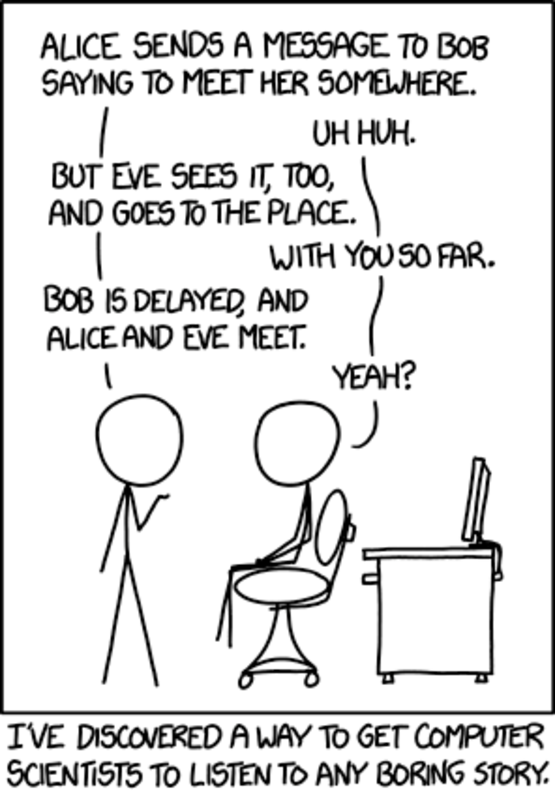
\includegraphics[width=45mm]{pic/alice-bob} 
\end{center}
\end{figure}
\end{frame}
\begin{frame}\frametitle{The Syntax of Encryption}
\begin{figure}
\begin{center}
\begin{tikzpicture}
\node (sender) [minimum size=1cm] {}; \Alice{0}{0}{0.4};
\node (bart) [below of = sender, node distance = 0.7cm] {Alice};
\node (enc) [draw, right of = sender, rounded corners=1ex,node distance = 2cm] {$\mathsf{Enc}$};
\node (k1) [above of = enc, node distance = 1cm] {$k$};
\node (c) [right of = enc, node distance = 2cm] {$c$};
\node (gen) [draw, above of = c, rounded corners=1ex,node distance = 1cm] {$\mathsf{Gen}$};
\node (adv) [below of = c, node distance = 1cm, minimum size=1cm] {}; \Evil{4cm}{-1cm}{0.4};
\node (burns) [below of = adv, node distance = 0.7cm] {Adversary};
\node (dec) [draw, right of = c, rounded corners=1ex,node distance = 2cm] {$\mathsf{Dec}$};
\node (k2) [above of = dec, node distance = 1cm] {$k$};
\node (receiver) [right of = dec, node distance = 2cm, minimum size=1cm] {}; \Bob{8cm}{0}{0.4};
\node (lisa) [below of = receiver, node distance = 0.7cm] {Bob};
\draw[-latex] (sender) -- (enc) node [midway, above] {$m$};
\draw (enc) -- (c); \draw[-latex] (c) -- (dec);
\draw[-latex] (dec) -- (receiver) node [midway, above] {$m$};
\draw[-latex] (k1) -- (enc);
\draw[-latex] (gen) -- (k1);
\draw[-latex] (gen) -- (k2);								
\draw[-latex] (k2) -- (dec);		
\end{tikzpicture}
\end{center}
\end{figure}
\begin{itemize}
\item key $k \in \mathcal{K}$, plaintext (or message) $m \in \mathcal{M}$, ciphertext $c \in \mathcal{C}$
\item \textbf{Key-generation} algorithm~$k \gets \mathsf{Gen}$
\item \textbf{Encryption} algorithm~$c:= \mathsf{Enc}_k(m)$
\item \textbf{Decryption} algorithm~$m:= \mathsf{Dec}_k(c)$
\item \textbf{Encryption scheme}: $\Pi = (\mathsf{Gen}, \mathsf{Enc}, \mathsf{Dec})$
\item \textbf{Basic correctness requirement}: $\mathsf{Dec}_k(\mathsf{Enc}_k(m)) = m$
\end{itemize}
\end{frame}
\begin{frame}\frametitle{Securing Key vs Obscuring Algorithm}
\begin{itemize}
\item Easier to maintain secrecy of a short key
\item In case the key is exposed, easier for the honest parties to change the key
\item In case many pairs of people, easier to use the same algorithm, but different keys
\end{itemize}
\begin{alertblock}{Kerckhoffs's principle}
\begin{quote}
The cipher method must not be required to be secret, and it must be able to fall into the hands of the enemy without inconvenience.
\end{quote}	
\end{alertblock}
\begin{alertblock}{Shannon's maxim}
	\begin{quote}
		The enemy knows the system.
	\end{quote}	
\end{alertblock}
\end{frame}
\begin{frame}\frametitle{Why ``Open Cryptographic Design''}
\begin{itemize}
\item Published designs undergo public scrutiny are to be stronger
\item Better for security flaws to be revealed by ``ethical hackers''
\item Reverse engineering of the code (or leakage by industrial espionage) poses a serious threat to security
\item Enable the establishment of standards.
\end{itemize}
\begin{exampleblock}{Dual EC: A Standardized Back Door}
	``Dual EC was standardized by NIST, ANSI, and ISO among other algorithms to generate pseudorandom numbers.'' ``The Snowden revelations, and in particular reports on Project Bullrun and the SIGINT Enabling Project, have indicated that Dual EC was part of a systematic effort by NSA to subvert standards.'' ``Reuters reported that NSA paid RSA ``\$10 million in a deal that set [Dual EC] as the preferred, or default, method for number generation in the BSafe software.''''	
\end{exampleblock}
\end{frame}
\begin{frame}\frametitle{Attack Scenarios}	
\begin{itemize}
\item \textbf{Ciphertext-only}: the adversary just observes ciphertext
\item \textbf{Known-plaintext}: the adversary learns pairs of plaintexts/ciphertexts under the same key
\item \textbf{Chosen-plaintext}: the adversary has the ability to obtain the encryption of plaintexts of its choice
\item \textbf{Chosen-ciphertext}: the adversary has the ability to obtain the decryption of \textbf{other} ciphertexts of its choice
\item \textbf{Passive attack}: COA KPA
\begin{itemize}
\item because not all ciphertext are confidential
\end{itemize}
\item \textbf{Active attack}: CPA CCA
\begin{itemize}
\item when to encrypt/decrypt whatever an adversary wishes?
\end{itemize}
\end{itemize}	
\end{frame}
\section{Historical Ciphers and Their Cryptanalysis}
\begin{comment}
	\begin{frame}\frametitle{Why We Learn Broken Ciphers?}
	\begin{itemize}
	\item To understand the weaknesses of an ``ad-hoc'' approach
	\item To learn that ``simple'' approaches are unlikely to succeed
	\item To feel that ``we are smart enough to do some crypt-analyzing''
	\end{itemize}
	\end{frame}
\end{comment}

\begin{frame}[fragile]\frametitle{Caesar's Cipher}
\begin{quote}
If he had anything confidential to say, he wrote it in cipher, that is, by so changing the order of the letters of the alphabet, that not a word could be made out. If anyone wishes to \alert{decipher} these, and get at their meaning, he must \alert{substitute the fourth letter of the alphabet, namely D, for A}, and so with the others

\rightline{--Suetonius,``Life of Julius Caesar''}
\end{quote}
\begin{itemize}
	\item $\mathsf{Enc}(m)=m+3\mod 26$ \footnote{In fact the quote indicates that decryption involved rotating letters of the alphabet forward 3 positions, $\mathsf{Dec}(c)=c+3\mod 26$}
	\item \textbf{Weakness}: ? %\alert{What is the key?}
\end{itemize}
\begin{exampleblock}{Example}
\verb|begintheattacknow|
%\verb|EHJLQWKHDWWDFNQRZ|
\end{exampleblock}
\end{frame}
\begin{frame}[fragile]\frametitle{Shift Cipher}
\begin{itemize}
\item $\mathsf{Enc}_k(m)=m+k\mod 26$
\item $\mathsf{Dec}_k(c)=c-k\mod 26$
\item \textbf{Weakness}: ? %Fragile under \textbf{Brute-force attack} (exhaustive search)
\end{itemize}
\begin{exampleblock}{Example: Decipher the string}	
\verb|EHJLQWKHDWWDFNQRZ|
\end{exampleblock}
\begin{alertblock}{Sufficient Key Space Principle}
Any secure encryption scheme must have a key space that is not vulnerable to exhaustive search.\footnote{If the plaintext space is larger than the key space.}
\end{alertblock}
\end{frame}
\begin{frame}\frametitle{Index of Coincidence (IC) Method (to find $k$)}
\textbf{How to automatically determine that the deciphered text makes sense?}

\textbf{Index of Coincidence (IC)}: the probability that two randomly selected letters (pick-then-return) will be identical.

Let $p_i$ denote the probability of $i$th letter in English text.
\[I \overset{\text{def}}{=}\sum_{i=0}^{25} p_i^2 \]
\begin{exampleblock}{Example}
What's the IC of `apple'?
\end{exampleblock}

For a long English text, the IC is $\approx 0.065$.
For $j = 0, 1, \dotsc , 25$, $q_j$ is the probability of $j$th letter in the ciphertext.
\[I_j \overset{\text{def}}{=}\sum_{i=0}^{25} p_i \cdot q_{i+j}\]
\alert{Q: For shift cipher, if $j = k$, then $I_j \approx$ ?}
\end{frame}

\begin{frame}[fragile]\frametitle{Mono-Alphabetic Substitution}
\begin{itemize}
\item \textbf{Idea}: To map each character to a different one in an arbitrary manner
\item \textbf{Strength}: Key space is large $\approx 2^{88}$. \alert{Q: how to count?}
\item \textbf{Weakness}: ? %The mapping of each letter is fixed
\end{itemize}
\begin{exampleblock}{Example}
\verb|abcdefghijklmnopqrstuvwxyz|\\
\verb|XEUADNBKVMROCQFSYHWGLZIJPT|

Plaintext: \verb|tellhimaboutme|\\
Ciphertext: \verb|??????????????|
\end{exampleblock}
\end{frame}
\begin{frame}[fragile]\frametitle{Attack with Statistical Patterns}
\begin{enumerate}
\item Tabulate the frequency of letters in the ciphertext
\item Compare it to those in English text
\item Guess the most frequent letter corresponds to \verb|e|, and so on
\item Choose the plaintext that does ``make sense'' (Not trivial)
\end{enumerate}
\begin{table}
\begin{center}
\caption{Average letter frequencies for English-language text}
\begin{tabular}{|cc|cc|cc|cc|cc|} \hline
e & 12.7\% & t & 9.1\% & a & 8.2\% & o & 7.5\% & i & 7.0\%\\
n & 6.7\% & \_ & 6.4\% & s & 6.3\% & h & 6.1\% & r & 6.0\%\\
d & 4.3\% & l & 4.0\% & c & 2.8\% & u & 2.8\% & m & 2.4\%\\
w & 2.4\% & f & 2.2\% & g & 2.0\% & y & 2.0\% & p & 1.9\%\\
b & 1.5\% & v & 1.0\% & k & 0.8\% & j & 0.2\% & x & 0.2\%\\
q & 0.1\% & z & 0.1\% & & & & & &\\ \hline
\end{tabular}
\end{center}
\end{table}
\end{frame}
\begin{frame}[fragile]\frametitle{Example of Frequency Analysis (Ciphertext)}
\begin{verbatim}
LIVITCSWPIYVEWHEVSRIQMXLEYVEOIEWHRXEXIPFEMVEWHKVS
TYLXZIXLIKIIXPIJVSZEYPERRGERIMWQLMGLMXQERIWGPSRIH
MXQEREKIETXMJTPRGEVEKEITREWHEXXLEXXMZITWAWSQWXSWE
XTVEPMRXRSJGSTVRIEYVIEXCVMUIMWERGMIWXMJMGCSMWXSJO
MIQXLIVIQIVIXQSVSTWHKPEGARCSXRWIEVSWIIBXVIZMXFSJX
LIKEGAEWHEPSWYSWIWIEVXLISXLIVXLIRGEPIRQIVIIBGIIHM
WYPFLEVHEWHYPSRRFQMXLEPPXLIECCIEVEWGISJKTVWMRLIHY
SPHXLIQIMYLXSJXLIMWRIGXQEROIVFVIZEVAEKPIEWHXEAMWY
EPPXLMWYRMWXSGSWRMHIVEXMSWMGSTPHLEVHPFKPEZINTCMXI
VJSVLMRSCMWMSWVIRCIGXMWYMX
\end{verbatim}
\end{frame}
\begin{frame}[fragile]\frametitle{Example of Frequency Analysis (Analysis)}
Count and Guess, Trial and Error.
\begin{table}
\begin{center}
\caption{Analysis Steps}
\begin{tabular}{|r|l|} \hline
Ciphertext & Plaintext \\ \hline
\alert{I}   & \alert{e} \\
\alert{XLI} & \alert{the} \\
\alert{E} & \alert{a} \\
\alert{R}tate & \alert{s}tate \\
atthatt\alert{MZ}e & atthatt\alert{im}e \\
he\alert{V}e & he\alert{r}e \\
remar\alert{A} & remar\alert{k} \\ \hline
\end{tabular}
\end{center}
\end{table}
\end{frame}
\begin{frame}[fragile]\frametitle{Example of Frequency Analysis (Plaintext)}
\begin{quote}
Hereupon Legrand arose, with a grave and stately air, and brought me the beetle
from a glass case in which it was enclosed. It was a beautiful scarabaeus, and, at
that time, unknown to naturalists -- of course a great prize in a scientific point
of view. There were two round black spots near one extremity of the back, and a
long one near the other. The scales were exceedingly hard and glossy, with all the
appearance of burnished gold. The weight of the insect was very remarkable, and,
taking all things into consideration, I could hardly blame Jupiter for his opinion
respecting it.

\rightline{--Edgar Allan Poe's ``The Gold-Bug''}
\end{quote}
\end{frame}

\begin{frame}[fragile]\frametitle{Vigen\`{e}re (poly-alphabetic shift) Cipher}
\begin{itemize}
\item \textbf{Idea}: To ``smooth out'' the distribution in the ciphertext by mapping different instances of the same letter in the plaintext to different ones in the ciphertext
\item \textbf{Encryption}: $c_i=m_i+k_{[i\bmod t]}$, $t$ is the length (period) of $k$
\item \textbf{Cryptanalysis}: Need find $t$; if $t$ is known, need know whether the decryption ``makes sense'', but brute force ($26^t$) is infeasible for $t > 15$
\end{itemize}
\begin{exampleblock}{Example (Key is `cafe')}
\begin{description}[Ciphertext]
\item[Plaintext]  \verb|tellhimaboutme| \\
\item[Key]        \verb|cafecafecafeca| \\
\item[Ciphertext] \verb|??????????????| %\verb|WFRQKJSFEPAYPF|
\end{description}
\end{exampleblock}
\end{frame}
\begin{frame}[fragile]\frametitle{Kasiski's Method (to find $t$)}
\begin{itemize}
\item To identify repeated patterns of length 2 or 3
\item The distance between such appearances is a multiple of $t$
\item $t$ is the greatest common divisor of all the distances
\end{itemize}
\begin{exampleblock}{Example (Key is `beads')}
\begin{semiverbatim}
themanandthewomanretrievedtheletterfromthepostoffice
beadsbeadsbeadsbeadsbeadsbeansdeadsbeadsbeadsbeadbea
VMFQTPFOH\alert{MJJ}XSFCSSIMTNFZXFYISEIYUIKHWPQ\alert{MJJ}QSLVTGJKGF
\end{semiverbatim}
\end{exampleblock}
\end{frame}
\begin{frame}\frametitle{Index of Coincidence (IC) Method (to find $t$)}
For $\tau = 1, 2, \dotsc$, $q_i$ is the probability of $i$th letter in $c_1, c_{1+\tau}, c_{1+2\tau}, \dotsc$, IC is
\[I_\tau \overset{\text{def}}{=}\sum_{i=0}^{25} q_i^2\]
\alert{If $\tau = t$, then $I_\tau \approx ?$} ; otherwise $q_i \approx \frac{1}{26}$ and
\[I_\tau \approx \sum_{i=0}^{25} \left(\frac{1}{26}\right)^2 \approx 0.038\]
Then reuse IC method to find $k_i$.
\begin{alertblock}{Arbitrary Adversary Principle}
Security must be guaranteed for any adversary within the class of adversaries having the specified power
\end{alertblock}
\end{frame}
\begin{frame}\frametitle{Cryptanalytic Attacks (homework assignment)}
\begin{itemize}
\item Under COA, the requirement for ciphertext related to the size of the key space.  Vig\`{e}nere > mono-alphabetic sub. > shift
\item Under KPA, trivially broken.
\end{itemize}
\begin{alertblock}{Lessons learned}
\begin{itemize}
\item Sufficient key space principle
\item Designing secure cipher is a hard task
\item Complexity does not imply security (then what does?)
\item Arbitrary adversary principle
\end{itemize}
\end{alertblock}
\end{frame}
\section{The Basic Principles of Modern Cryptography}
\begin{frame}\frametitle{Three Main Principles of Modern Cryptography}
\begin{enumerate}
\item The formulation of a rigorous \textbf{definition} of security / threat model
\item When the security of a cipher relies on an unproven \textbf{assumption}, this assumption must be precisely stated and be as minimal as possible
\item Cipher should be accompanied by a rigorous \textbf{proof} of security with the above definition and the above assumption
\end{enumerate}
\end{frame}
\begin{frame}\frametitle{Why Principle 1 -- Formulation of Exact Definitions}
\begin{exampleblock}{Q: how would you formalize the security for private-key encryption?}
\begin{enumerate}
\item \emph{No adversary can find the secret key when given a ciphertext.}\\
$\mathsf{Enc}_k(m)=m$
\item \emph{No adversary can find the plaintext that corresponds to the ciphertext.}\\
$\mathsf{Enc}_k(m)=m_{0}\| \mathsf{AES}_k(m)$
\item \emph{No adversary can determine any character of the plaintext that corresponds to the ciphertext.}\\
$m=1000$, someone can learn $ 800 < m < 1200$
\item \emph{No adversary can derive any meaningful information about the plaintext from the ciphertext.}\\
Could you define so-called `meaningful'?
\end{enumerate}
\emph{\alert{Definitions of security should suffice for all potential applications.}}
\end{exampleblock}
\end{frame}
\begin{frame}\frametitle{Why Principle 1 -- How to define}
%\begin{exampleblock}{General Form}
%A cryptographic scheme for a given \textbf{task} is secure if no adversary of a specified \textbf{power} can achieve a specified \textbf{break}
%\end{exampleblock}

How To Define Security -- Lesson From Alan Turing
\begin{itemize}
\item What's computation?\footnote{Q: Any ``mathematical proof that there exist well-defined problems that computers cannot solve''? A: Halting Problem in computability theory}
\begin{enumerate}
\item A direct appeal to \textbf{intuition}
\item A \textbf{proof of the equivalence} of two definitions\\ (The new one has a greater intuitive appeal)
\item Giving \textbf{examples} solved using a definition
\end{enumerate}
\item Additional method for security: \textbf{Test of time}
\end{itemize}
\end{frame}	
\begin{frame}\frametitle{Principle 2 -- Reliance on Precise Assumptions}
Most cryptographic constructions \textbf{cannot be proven secure unconditionally}
\begin{itemize}
	\item \textbf{Why?} 
	\begin{enumerate}
		\item Validation of the assumption
		\item Comparison of schemes
		\item Facilitation of proofs of security
	\end{enumerate}
	\textbf{The construction is secure if the assumption is true.}
	\item \textbf{How?} 
	\begin{enumerate}
		\item old, so well tested
		\item simple and lower-level, so easy to study, refute \& correct
	\end{enumerate}
\end{itemize}
\end{frame}
\begin{frame}\frametitle{Principle 3 -- Rigorous Proofs of Security}
\begin{itemize}
\item \textbf{Why?} Proofs are more desirable in computer security than in other fields.
\item \textbf{The reductionist approach}: 
\begin{theorem}	Given that Assumption X is true, Construction Y is secure according to the given definition.
\end{theorem}
\begin{proof} Reduce the problem given by X to the problem of breaking Y.
\end{proof}
\item \textbf{Ad-hoc approaches}: for those who need a ``quick and dirty'' solution, or who are just simply unaware.
\end{itemize}
\end{frame}
\begin{frame}\frametitle{Summary}
\begin{itemize}
\item Cryptography secures information, transactions and computations
\item Kerckhoffs's principle \& Open cryptographic design
\item Caesar's, shift, Mono-Alphabetic sub., Vigen\`{e}re
\item Brute force, letter frequency, Kasiski's, IC
\item Sufficient key space principle
\item Arbitrary adversary principle
\item Rigorously proven security
\end{itemize}
\end{frame}
\end{document}


%% presentation
\documentclass{beamer}
\usetheme[height=7mm]{Rochester}
\usecolortheme{rose}

% handout

%\documentclass[handout]{beamer}
%\usepackage{pgfpages} \pgfpagesuselayout{8 on 1}[a4paper]

%\documentclass[mathserif]{article}
%\usepackage{beamerarticle}

\usepackage{amsmath}
\usepackage{comment}
\usepackage{amssymb,amsfonts}
\usepackage[T1]{fontenc}
\usepackage{lmodern}
\usepackage{tikz}
%\usepackage{simpsons}
\usepackage{marvosym}
\usepackage{color}
\usepackage{multirow}
\usepackage{pgffor}
\usepackage{pgfplots}
\usepackage[slide,algoruled,titlenumbered,vlined,noend,linesnumbered,]{algorithm2e}

\usefonttheme{structurebold}

\setbeamertemplate{footline}[frame number]
\setbeamertemplate{navigation symbols}{}
\setbeamerfont{smallverb}{size*={73}}
\usefonttheme[onlymath]{serif}
\setbeamertemplate{theorems}[numbered]
\newtheorem{construction}[theorem]{Construction}
\newtheorem{proposition}[theorem]{Proposition}

\AtBeginSection[] {
  \begin{frame}
    \frametitle{Content}
    \tableofcontents[currentsection]
  \end{frame}
  \addtocounter{framenumber}{-1}
}

\usetikzlibrary[shapes.arrows]
\usetikzlibrary{shapes.geometric}
\usetikzlibrary{backgrounds}
\usetikzlibrary{positioning}
\usetikzlibrary{calc}
\usetikzlibrary{intersections}
\usetikzlibrary{fadings}
\usetikzlibrary{decorations.footprints}
\usetikzlibrary{patterns}
\usetikzlibrary{shapes.callouts}
\usetikzlibrary{fit}
%handout

\providecommand{\abs}[1]{\lvert#1\rvert}

\tikzset{every picture/.style={line width=1pt,show background rectangle},background rectangle/.style={fill=blue!10,rounded corners=2ex}}

\newcommand{\Bob}[3]{ \begin{scope}[shift={(#1,#2)},scale=#3]
  \draw (0,0) circle (0.95 and 1);
  \fill (-0.3,-0.1) circle (0.1);
  \fill (+0.3,-0.1) circle (0.1);
  \draw (0.35,-0.5) arc (-70:-110: 1 and 0.4);
  \draw (-0.3,0.5) arc (-10:-80: 0.8 and 0.8);
  \draw (-0.5,0.8) arc (190:255: 2 and 1);
  \draw (-0.7,0.9) -- +(0.2,-0.09) -- +(0.25,0.2);
  \end{scope} }

\newcommand{\Alice}[3]{ \begin{scope}[shift={(#1,#2)},scale=#3]
  \draw (0,0) circle (0.95 and 1);
  \fill (-0.3,-0.1) circle (0.1);
  \fill (+0.3,-0.1) circle (0.1);
  \draw (0.35,-0.5) arc (-70:-110: 1 and 0.4);
  \draw (0.3,1.3) arc (20:-100: 1.4 and 1);
  \draw (0.5,1.3) arc (150:260: 1 and 1);
  \draw (0.41,1.3) circle (0.35);
  \end{scope} }

  \newcommand{\Evil}[3]{ \begin{scope}[shift={(#1,#2)},scale=#3]
    \draw (0,0) circle (0.95 and 1);
    \fill (-0.1,-0.1) -- +(-0.2,-0.1) -- +(-0.4,0.2); %eye
    \fill (0.1,-0.1) -- +(0.2,-0.1) -- +(0.4,0.2);
    \draw (0.35,-0.5) arc (-70:-110: 1 and 0.4);
    %\fill (0.3,-0.5) -- +(-0.1,-0.2) -- +(-0.2,-0.02);
    %\fill (-0.3,-0.5) -- +(0.1,-0.2) -- +(0.2,-0.02);
    \fill (0.3,0.7) -- +(0.5,0.4) -- +(0.4,-0.2); % horn
    \fill (-0.3,0.7) -- +(-0.5,0.4) -- +(-0.4,-0.2);
    %\draw (0.3,1.3) arc (20:-100: 1.4 and 1);
    %\draw (0.5,1.3) arc (150:260: 1 and 1);
    %\draw (0.41,1.3) circle (0.35);
    \end{scope} }

\newcommand{\Charlie}[3]{ \begin{scope}[shift={(#1,#2)},scale=#3]
    \draw (0,0) circle (0.95 and 1);
    \filldraw[fill=black!20] (-0.35,-0.1) circle (0.25);
    \filldraw[fill=black!20] (+0.35,-0.1) circle (0.25);
    %\draw (0.9,0.2) to [bend left] (-0.9,0.2);
    \draw (0.2,0) to [bend left] (-0.2,0);


    %\draw (0.3,0.7) to [bend right] (-0.3,0.7);
    %\draw (0.4,0.5) to [bend right] (-0.4,0.5);
    %\draw (0.35,-0.5) arc (-70:-110: 1 and 0.4);
    \draw (-0.7,-0.6) to [bend right] (0,-0.6) to [bend right] (0.7,-0.6) to [bend right]  (0,-0.5)  to [bend right]  cycle ;
    %\draw (0.3,1.3) arc (20:-100: 1.4 and 1);
    %\draw (0.5,1.3) arc (150:260: 1 and 1);
    %\draw (0.41,1.3) circle (0.35);
    \end{scope} }

\author{Yu Zhang}
\institute{Harbin Institute of Technology}
\date[Crypto'22A]{Cryptography, Autumn, 2022}

%\input{1introduction.tex}
%\input{2perfectlysecret.tex}
%\input{3privatekey.tex}


\title{Perfectly Secret Encryption}

\begin{document}
\maketitle
\begin{frame}\frametitle{Outline}
\tableofcontents
\end{frame}
\section{Definitions and Basic Properties}
\begin{frame}\frametitle{Recall The Syntax of Encryption}
\begin{figure}
\begin{center}
\begin{tikzpicture}
\node (sender) [minimum size=1cm] {}; \Alice{0}{0}{0.4};
\node (bart) [below of = sender, node distance = 0.7cm] {Alice};
\node (enc) [draw, right of = sender, rounded corners=1ex,node distance = 2cm] {$\mathsf{Enc}$};
\node (k1) [above of = enc, node distance = 1cm] {$k$};
\node (c) [right of = enc, node distance = 2cm] {$c$};
\node (gen) [draw, above of = c, rounded corners=1ex,node distance = 1cm] {$\mathsf{Gen}$};
\node (adv) [below of = c, node distance = 1cm, minimum size=1cm] {}; \Evil{4cm}{-1cm}{0.4};
\node (burns) [below of = adv, node distance = 0.7cm] {Adversary};
\node (dec) [draw, right of = c, rounded corners=1ex,node distance = 2cm] {$\mathsf{Dec}$};
\node (k2) [above of = dec, node distance = 1cm] {$k$};
\node (receiver) [right of = dec, node distance = 2cm, minimum size=1cm] {}; \Bob{8cm}{0}{0.4};
\node (lisa) [below of = receiver, node distance = 0.7cm] {Bob};
\draw[-latex] (sender) -- (enc) node [midway, above] {$m$};
\draw (enc) -- (c); \draw[-latex] (c) -- (dec);
\draw[-latex] (dec) -- (receiver) node [midway, above] {$m$};
\draw[-latex] (k1) -- (enc);
\draw[-latex] (gen) -- (k1);
\draw[-latex] (gen) -- (k2);								
\draw[-latex] (k2) -- (dec);		
\end{tikzpicture}
\end{center}
\end{figure}
\begin{itemize}
\item $k \in \mathcal{K}, m \in \mathcal{M}, c \in \mathcal{C}$.
\item $k \gets \mathsf{Gen}, c:= \mathsf{Enc}_k(m), m:= \mathsf{Dec}_k(c)$.
\item \textbf{Encryption scheme}: $\Pi = (\mathsf{Gen}, \mathsf{Enc}, \mathsf{Dec})$.
\item \textbf{Random Variable}: $K, M, C$ for key, plaintext, ciphertext.
\item \textbf{Probability}: $\Pr[K=k], \Pr[M=m], \Pr[C=c].$
\item \alert{What's the basic correctness requirement?}
\end{itemize}
\end{frame}
\begin{frame}\frametitle{Definition of `Perfect Secrecy'}
\textbf{Intuition}: An adversary knows the probability distribution over $\mathcal{M}$. $c$ should have no effect on the knowledge of the adversary; the a \emph{posteriori} likelihood that some $m$ was sent should be no different from the a \emph{priori} probability that $m$ would be sent. 
\begin{definition}
$\Pi$ over $\mathcal{M}$ is \textbf{perfectly secret} if for every probability distribution over $\mathcal{M}$, $\forall m \in \mathcal{M}$ and $\forall c \in \mathcal{C}$ for which $\Pr[C = c] > 0$:
\[ \Pr[M=m | C=c] = \Pr[M=m].\]
\end{definition}
\textbf{Simplify}: non-zero probabilities for $\forall m \in \mathcal{M}$ and $\forall c \in \mathcal{C}$.\\

\begin{exampleblock}{Is the below scheme perfectly secret?}{ For $\mathcal{M}=\mathcal{K} = \{ 0,1 \} , \mathsf{Enc}_k(m)= m \oplus k$.}\end{exampleblock}
\end{frame}

\begin{frame}\frametitle{Perfect Secrecy On One Bit}

\begin{exampleblock}{XORing one bit is perfectly secret.}
Let $\Pr[M=1] = p$ and $\Pr[M=0] = 1-p$.
Let us consider a case that $M=1$ and $C=1$.
\[ \Pr[M=1 | C=1] = \Pr[C=1 | M=1 ] \cdot \Pr[ M=1 ] / \Pr[C=1] \]
\[ = \frac{\Pr[K = 1\oplus 1] \cdot p }{ \Pr[C=1 | M=1] \cdot \Pr[M=1] + \Pr[C=1 | M=0] \cdot \Pr[M=0]} \]
\[ = \frac{1/2 \cdot p }{ 1/2 \cdot p + 1/2 \cdot (1-p)} = p = \Pr[M=1] \]
We can do the same for other cases.
\end{exampleblock}
Note that $\Pr[M=1 | C=1] \neq \Pr[M=1, C=1] = \Pr[C=1 | M=1] \cdot \Pr[M=1] = 1/2 \cdot p$.
\end{frame}

\begin{frame}\frametitle{An Equivalent Formulation}
\begin{lemma} \label{lem:ps} 
$\Pi$ over $\mathcal{M}$ is perfectly secret $\iff$ for every probability distribution over $\mathcal{M}$, $\forall m \in \mathcal{M}$ and $\forall c \in \mathcal{C}$:
\[ \Pr[C=c | M=m] = \Pr[C=c].\]
\end{lemma}
\begin{proof}
$\Leftarrow$: Multiplying both sides by $\Pr[M=m]/\Pr[C=c]$, then use Bayes' Theorem.\footnote{If $\Pr[B]\neq 0$ then $ \Pr[A|B] = \left( \Pr[A] \cdot \Pr[B|A] \right) / \Pr[B] $} \\
$ \Pr[C=c | M=m] \cdot \Pr[M=m] / \Pr[C=c] = \Pr[M=m]$\\
$ \Pr[M=m | C=c] \cdot \Pr[C=c] / \Pr[C=c] = \Pr[M=m | C=c]$
$\Rightarrow$: Multiplying both sides by $\Pr[C=c]/\Pr[M=m]$, then use Bayes' Theorem.
\end{proof}
\end{frame}
\begin{frame}\frametitle{Perfect Indistinguishability}
\begin{lemma}\label{lem:pi}
$\Pi$ over $\mathcal{M}$ is perfectly secret $\iff$ for every probability distribution over $\mathcal{M}$, $\forall m_0, m_1 \in \mathcal{M}$ and $\forall c \in \mathcal{C}$:
\[ \Pr[C=c | M=m_0] = \Pr[C=c | M=m_1].\]
\end{lemma}
\begin{proof}
$\Rightarrow$: By Lemma \ref{lem:ps}: $\Pr[C=c | M=m] = \Pr[C=c]$. \\
$\Leftarrow$: $p \overset{\text{def}}{=} \Pr[C=c | M=m_0]$.
\[
\begin{split}
	\Pr[C=c] &= \sum_{m \in \mathcal{M}} \Pr[C=c|M=m] \cdot \Pr[M=m] \\
	&= \sum_{m \in \mathcal{M}} p \cdot \Pr[M=m] = p = \Pr[C=c|M=m_0].
\end{split}
\]
\end{proof}
\end{frame}
\section{The One-Time Pad (Vernam's Cipher)}
\begin{frame}\frametitle{One-Time Pad (Vernam's Cipher)}
\begin{itemize}
	\item $\mathcal{M} = \mathcal{K} = \mathcal{C} = \{0,1\}^{\ell}$.
	\item $\mathsf{Gen}$ chooses a $k$ randomly with probability exactly $2^{-\ell}$.
	\item $c := \mathsf{Enc}_k(m) = k \oplus m$. 
	\item $m := \mathsf{Dec}_k(c) = k \oplus c$. 
\end{itemize}
\begin{theorem}
The one-time pad encryption scheme is perfectly-secret.
\end{theorem}
\begin{proof}
\[\begin{split} \Pr[C=c|M=m] &= \Pr[M \oplus K=c|M=m] \\
&= \Pr[m \oplus K=c] = \Pr[K = m \oplus c] = 2^{-\ell}.
\end{split}
\]
Then Lemma \ref{lem:pi}: $\Pr[C=c | M=m_0] = \Pr[C=c | M=m_1]$.
\end{proof}
\end{frame}
\section{Limitations of Perfect Secrecy}
\begin{frame}\frametitle{Limitations of OTP and Perfect Secrecy}
Key $k$ is as long as $m$, difficult to store and share $k$.
\begin{theorem}
Let $\Pi$ be perfectly-secret over $\mathcal{M}$, and let $\mathcal{K}$ be determined by $\mathsf{Gen}$. Then $|\mathcal{K}|\ge |\mathcal{M}|$. 
\end{theorem}
\begin{proof}
Assume $|\mathcal{K}| < |\mathcal{M}|$.
$\mathcal{M}(c) \overset{\text{def}}{=} \{ \hat{m} | \hat{m} = \mathsf{Dec}_k(c)\  \text{for some}\ \hat{k} \in \mathcal{K} \}$. Since for one $k$, there is at most one $m$ such that $m = \mathsf{Dec}_k(c)$, $|\mathcal{M}(c)|\le |\mathcal{K}| < |\mathcal{M}|$. So $\exists m' \notin \mathcal{M}(c)$. Then
\[ \Pr[M=m'|C=c] = 0 \neq \Pr[M = m'] \]
and so not perfectly secret.
\end{proof}
\end{frame}
\begin{frame}\frametitle{Two Time Pad: Real World Cases}
Only used once for the same key, otherwise
\[c\oplus c'=(m\oplus k)\oplus (m'\oplus k)=m\oplus m'.\]
Learn $m$ from $m\oplus m'$ due to the redundancy of language.
\begin{exampleblock}{MS-PPTP (Win NT)}
\begin{figure}
\begin{center}
\begin{tikzpicture}
\node (sender) [minimum size=1cm,label=below:Client, label=above:$k$] {}; \Alice{0}{0}{0.4};
\node (c) at ($(sender)+(4cm,0.5cm)$) {$\left[ m_1\|m_2\|m_3\right] \oplus PRG(k)$};
\node (c1) [below of = c, node distance = 1cm] {$\left[s_1\|s_2\|s_3\right] \oplus PRG(k)$};
\node (receiver) at ($(sender)+(8cm,0)$) [minimum size=1cm,label=below:Server, label=above:$k$] {}; \Bob{8cm}{0}{0.4};
\draw[-latex] (sender.east |- c) -- (c) -- (receiver.west |- c);
\draw[-latex] (receiver.west |- c1) -- (c1) -- (sender.east |- c1);
\end{tikzpicture}
\end{center}
\end{figure}
Improvement: use two keys for C-to-S and S-to-C separately.
\end{exampleblock}
\end{frame}
\section{Shannon's Theorem}
\begin{frame}\frametitle{Shannon's Theorem}
\begin{theorem}
For $|\mathcal{M}| = |\mathcal{K}| = |\mathcal{C}|$, $\Pi$ is perfectly secret $\iff$
\begin{enumerate}
\item Every $k \in \mathcal{K}$ is chosen with probability $1/|\mathcal{K}|$ by $\mathsf{Gen}$.
\item $\forall m \in \mathcal{M}$ and $\forall c \in \mathcal{C}$, $\exists$ unique $k \in \mathcal{K}$: $c := \mathsf{Enc}_k(m)$.
\end{enumerate}
\end{theorem}
\begin{proof}
$\Leftarrow$: $\Pr[C=c|M=m]=1/|\mathcal{K}|$, use Lemma \ref{lem:pi}. \\
$\Rightarrow (2)$: At least one $k$, otherwise $\Pr[C=c|M=m]=0$; \\
at most one $k$, because $\{\mathsf{Enc}_k(m)\}_{k\in \mathcal{K}} = \mathcal{C}$ and $|\mathcal{K}| = |\mathcal{C}|$.\\
$\Rightarrow (1)$: $k_i$ is such that $\mathsf{Enc}_{k_i}(m_i)=c$.
\[ \begin{split}
\Pr[M = m_i] &= \Pr[M=m_i|C=c] \\
             &= \left( \Pr[C =c|M=m_i] \cdot \Pr[M = m_i] \right) / \Pr[C=c] \\
 &= \left( \Pr[K=k_i] \cdot \Pr[M = m_i] \right) / \Pr[C=c],
\end{split}
\]
so $\Pr[K=k_i] = \Pr[C = c] = 1/|\mathcal{K}|$.
\end{proof}
\end{frame}

\begin{frame}\frametitle{Application of Shannon's Theorem}
\begin{exampleblock}{Is the below scheme perfectly secret?}
Let $\mathcal{M} = \mathcal{C} = \mathcal{K} = \{ 0, 1, 2,\dots , 255 \} $\\
$\mathsf{Enc}_k(m) = m  + k \mod 256$\\
$\mathsf{Dec}_k(c) = c - k \mod 256$
\end{exampleblock}
\end{frame}
\section{Eavesdropping Indistinguishability}
\begin{frame}\frametitle{Eavesdropping Indistinguishability Experiment}
$\mathsf{PrivK}^{\mathsf{eav}}_{\mathcal{A},\Pi}$ denote a \textbf{priv}ate-\textbf{k}ey encryption experiment for a given $\Pi$ over $\mathcal{M}$ and an \textbf{eav}esdropping adversary $\mathcal{A}$.
\begin{enumerate}
	\item $\mathcal{A}$ outputs a pair of messages $m_0, m_1 \in \mathcal{M}$.
	\item $k \gets \mathsf{Gen}$, a random bit $b \gets \{0,1\}$ is chosen. Then $c \gets \mathsf{Enc}_k(m_b)$ is given to $\mathcal{A}$.
	\item $\mathcal{A}$ outputs a bit $b'$
	\item If $b' = b$, $\mathcal{A}$ succeeded $\mathsf{PrivK}^{\mathsf{eav}}_{\mathcal{A},\Pi}=1$, otherwise 0.
\end{enumerate}
\begin{figure}
\begin{center}
\begin{tikzpicture}
%\node (A) at (0,0) {\Homer};
%\node (B) [right of = A, node distance = 4cm] {\Left\Burns};
\node (A) at (0,0) [minimum size=1cm] {}; \Charlie{0}{0}{0.4};
\node (B) [right of = A, node distance = 4cm, minimum size=1cm] {}; \Evil{4cm}{0}{0.4};
\node (1a) [below of=A, node distance=1cm] {};
\node (1b) [below of=B, node distance=1cm] {$m_0, m_1$};
\draw[-latex] (1b) -- (1a) node [midway,above] {};
\node (2a) [below of=1a, node distance=0.5cm] {Gen $b, k$};
\node (2b) [below of=1b, node distance=0.5cm] {};
%\draw[-latex] (2b) -- (2a) node [midway,above] {};
%\node (3a) [below of=2a, node distance=0.5cm] {};
%\node (3b) [below of=2b, node distance=0.5cm] {};
\node (4a) [below of=2a, node distance=0.5cm] {$\mathsf{Enc}_k(m_b)$};
\node (4b) [below of=2b, node distance=0.5cm] {};
\draw[-latex] (4a) -- (4b) node [midway,above] {};
\node (5a) [below of=4a, node distance=0.5cm] {};
\node (5b) [below of=4b, node distance=0.5cm] {$b'$};
\draw[-latex] (5b) -- (5a) node [midway,above] {};
\node (6a) [below of=5a, node distance=0.5cm] {};
\node (6b) [below of=5b, node distance=0.5cm] {};
\node (result) [right of = 6a, node distance = 2cm] {Win if $b = b'$};
\end{tikzpicture}

\end{center}
\end{figure}
\end{frame}
\begin{frame}\frametitle{Adversarial Indistinguishability}
\begin{definition}
$\Pi$ over $\mathcal{M}$ is \textbf{perfectly secret} if for every $\mathcal{A}$ it holds that
\[ \Pr[\mathsf{PrivK}^{\mathsf{eav}}_{\mathcal{A},\Pi}=1] = \frac{1}{2}.\]
\end{definition}
\begin{exampleblock}{Which in the below schemes are perfectly secret?}
\begin{itemize}
\item $\mathsf{Enc}_{k,k'}(m)= \mathsf{OTP}_k(m) \| \mathsf{OTP}_{k'}(m)$
\item $\mathsf{Enc}_{k}(m)= reverse(\mathsf{OTP}_k(m))$
\item $\mathsf{Enc}_{k}(m)= \mathsf{OTP}_k(m) \| k$
%To break semantic security, an attacker would read the secret key from the challenge ciphertext and use it to decrypt the challenge ciphertext. Basically, any ciphertext reveals the secret key.
\item $\mathsf{Enc}_{k}(m)= \mathsf{OTP}_k(m) \| \mathsf{OTP}_k(m) $
\item $\mathsf{Enc}_{k}(m)= \mathsf{OTP}_{0^{n}}(m)$
%To break semantic security, an attacker would ask for the encryption of $0^n$ and $1^n$ and can easily distinguish EXP(0) from EXP(1) because it knows the secret key, namely 0n.
\item $\mathsf{Enc}_{k}(m)= \mathsf{OTP}_k(m) \| LSB(m)$
%To break semantic security, an attacker would ask for the encryption of $0^n$ and $0^{n-1}1$ and can distinguish EXP(0) from EXP(1).
\end{itemize}
\end{exampleblock}
\end{frame}

\begin{frame}\frametitle{Summary}
\begin{itemize}
\item Perfect secrecy $=$ Perfect indistinguishability $=$ Adversarial indistinguishability
\item Perfect secrecy is attainable. The One-Time Pad (Vernam's cipher)
\item Shannon's theorem
\end{itemize}	
\end{frame}
\end{document}

%\input{3privatekey.tex}

\title{CCA-Secure and Authentication Encryption}
\begin{document}
\maketitle
\begin{frame}
\frametitle{Outline}
\tableofcontents
\end{frame}
\section{Authenticated Encryptions}
\begin{frame}\frametitle{Recall Security Against CCA}
The CCA indistinguishability experiment $\mathsf{PrivK}^{\mathsf{cca}}_{\mathcal{A},\Pi}(n)$:
\begin{enumerate}
	\item $k \gets \mathsf{Gen}(1^n)$.
	\item $\mathcal{A}$ is given input $1^n$ and oracle access $\mathcal{A}^{\mathsf{Enc}_k(\cdot)}$ and $\mathcal{A}^{\mathsf{Dec}_k(\cdot)}$, outputs $m_0, m_1$ of the same length.
	\item a random bit $b \gets \{0,1\}$ is chosen. Then $c \gets \mathsf{Enc}_k(m_b)$ is given to $\mathcal{A}$.
	\item $\mathcal{A}$ continues to have oracle access \textbf{except for $c$}, outputs $b'$.
	\item If $b' = b$, $\mathcal{A}$ succeeded $\mathsf{PrivK}^{\mathsf{cca}}_{\mathcal{A},\Pi}=1$, otherwise 0.
\end{enumerate}
\begin{definition}
$\Pi$ has \textbf{indistinguishable encryptions under a CCA (CCA-secure)} if $\forall$ \textsc{ppt} $\mathcal{A}$, $\exists$ $\mathsf{negl}$ such that
\[ \Pr\left[\mathsf{PrivK}^{\mathsf{cca}}_{\mathcal{A},\Pi}(n)=1\right] \le \frac{1}{2} + \mathsf{negl}(n).
\]
\end{definition}
\end{frame}
\begin{frame}\frametitle{Message Transmission Scheme}
\begin{figure}
\begin{center}
\begin{tikzpicture}
\node (sender) [minimum size=1cm] {}; \Alice{0}{0}{0.4};
\node (bart) [below of = sender, node distance = 0.7cm] {Alice};
\node (enc) [draw, right of = sender, rounded corners=1ex,node distance = 2cm] {$\mathsf{EncMac}'$};
\node (k1) [above of = enc, node distance = 1cm] {$k$};
\node (c) [right of = enc, node distance = 2cm] {$c$};
\node (gen) [draw, above of = c, rounded corners=1ex,node distance = 1cm] {$\mathsf{Gen}'$};
\node (adv) [below of = c, node distance = 1cm, minimum size=1cm] {}; \Evil{4cm}{-1cm}{0.4};
\node (burns) [below of = adv, node distance = 0.7cm] {Adversary};
\node (dec) [draw, right of = c, rounded corners=1ex,node distance = 2cm] {$\mathsf{Dec}'$};
\node (k2) [above of = dec, node distance = 1cm] {$k$};
\node (receiver) [right of = dec, node distance = 2cm, minimum size=1cm] {}; \Bob{8cm}{0}{0.4};
\node (lisa) [below of = receiver, node distance = 0.7cm] {Bob};
\draw[-latex] (sender) -- (enc) node [midway, above] {$m$};
\draw (enc) -- (c); \draw[-latex] (c) -- (dec);
\draw[-latex] (dec) -- (receiver) node [midway, above] {$m$};
\draw[-latex] (k1) -- (enc);
\draw[-latex] (gen) -- (k1);
\draw[-latex] (gen) -- (k2);								
\draw[-latex] (k2) -- (dec);
\node (perp) [below of=dec, node distance = 1.5cm] {$\perp$};
\draw[dotted,-latex] (adv) -- (dec);
\draw[dotted,-latex] (dec) -- (perp);
\end{tikzpicture}
\end{center}
\end{figure}
\begin{itemize}
\item \textbf{Key-generation} algorithm outputs $k \gets \mathsf{Gen'}(1^n)$. $k = (k_1,k_2)$. $k_1 \gets \mathsf{Gen}_E(1^n)$, $k_2 \gets \mathsf{Gen}_M(1^n)$.
\item \textbf{Message transmission} algorithm is derived from $\mathsf{Enc}_{k_1}(\cdot)$ and $\mathsf{Mac}_{k_2}(\cdot)$, outputs $c \gets \mathsf{EncMac'}_{k_1,k_2}(m)$. 
\item \textbf{Decryption} algorithm is derived from $\mathsf{Dec}_{k_1}(\cdot)$ and $\mathsf{Vrfy}_{k_2}(\cdot)$, outputs $m \gets \mathsf{Dec}'_{k_1,k_2}(c)$ or $\bot$.
\item \textbf{Correctness requirement}: $\mathsf{Dec}'_{k_1,k_2}(\mathsf{EncMac}'_{k_1,k_2}(m)) = m$.
\end{itemize}
\end{frame}
\begin{frame}\frametitle{Defining Secure Message Transmission}
The secure message transmission experiment $\mathsf{Auth}_{\mathcal{A},\Pi'}(n)$:
\begin{enumerate}
\item $k = (k_1,k_2) \gets \mathsf{Gen}'(1^n)$.
\item $\mathcal{A}$ is given input $1^n$ and oracle access to $\mathsf{EncMac'}_k$, and outputs $c \gets \mathsf{EncMac'}_{k}(m)$.
\item $m := \mathsf{Dec}'_k(c)$. $\mathsf{Auth}_{\mathcal{A},\Pi'}(n) = 1 \iff m \ne \bot \land\; m \notin \mathcal{Q}$.
\end{enumerate}
\begin{definition}
$\Pi'$ achieves \textbf{authenticated communication} if $\forall$ \textsc{ppt} $\mathcal{A}$, $\exists\; \mathsf{negl}$ such that
\[ \Pr[\mathsf{Auth}_{\mathcal{A},\Pi'}(n) = 1] \le \mathsf{negl}(n).
\]
\end{definition}
\begin{definition}
$\Pi'$ is \textbf{secure Authenticated Encryption (A.E.)} if it is both CCA-secure and also achieves authenticated communication.%\footnote{CPA security and integrity imply CCA security.}
\end{definition}
\begin{alertblock}{Does CCA-security imply A.E.? (homework)}
\end{alertblock}
\end{frame}
\begin{frame}\frametitle{Questions}
\begin{exampleblock}{Suppose $(E, D)$ provides A.E. Which of the following systems provide A.E.? }
\begin{itemize}
\item $E'_{k}(m) = \left( E_{k}(m), E_{k}(m)\right)$ and $D'_{k}(c_{1}, c_{2}) = D_{k}(c_{1})$ %n
\item $E'_{k}(m) = \left( E_{k}(m), 0\right)$ and %y
$ D'_{k}(c, b) = \left\{ 
  \begin{array}{l l}
    D_{k}(c) & \quad \text{if $b = 0$}\\
    \perp & \quad \text{otherwise}\\
  \end{array} \right. $
%\item $E'_{k}(m) = E_{k}(m)\oplus1^*$ and $D'_{k}(c) = D_{k}(c\oplus 1^{*})$ %y
\item $E'_{k}(m) = \left( E_{k}(m), E_{k}(m)\right)$ and %n E?(k,m)=(c1,c2) will output c1 != c2. The attacker then outputs (c1,c1)
$ D'_{k}(c_{1}, c_{2}) = \left\{ 
  \begin{array}{l l}
    D_{k}(c_{1}) & \ \text{if $D_{k}(c_{1}) = D_{k}(c_{2})$}\\
    \perp & \ \text{otherwise}\\
  \end{array} \right. $
\item $E'_{k}(m) = \left( E_{k}(m), H(m)\right)$ ($H$ is a CRHF) and %n H leaks m.
$ D'_{k}(c, h) = \left\{ 
  \begin{array}{l l}
    D_{k}(c) & \ \text{if $H(D_{k}(c))=h$}\\
    \perp & \ \text{otherwise}\\
  \end{array} \right. $ 
\end{itemize}
\end{exampleblock}
\end{frame}
\begin{frame}\frametitle{Combining Encryption and Authentication}
\begin{figure}
\begin{center}
\begin{tikzpicture}
\node (enc1) [minimum width=1.5cm, minimum height=1.5cm, draw] {$\mathsf{Enc}$};
\node (mac1) [right of=enc1, minimum width=1.5cm, minimum height=1.5cm, node distance=1.5cm, draw] {$\mathsf{Mac}$};	

\node (enc2) [right of=mac1, node distance=3cm, minimum width=3cm, minimum height=1.5cm, draw] {};
\node (mac2) [right of=enc2, minimum width=1.5cm, minimum height=1cm, node distance=0.75cm, draw] {$\mathsf{Mac}$};
\node (enc4) [left of=enc2, minimum width=1cm, minimum height=1cm, node distance=0.75cm] {$\mathsf{Enc}$}; 

\node (mac3) [right of=mac2, node distance=3cm, minimum width=3cm, minimum height=1.5cm, draw] {};
\node (enc3) [right of=mac3, minimum width=1.5cm, minimum height=1cm, node distance=0.75cm, draw] {$\mathsf{Enc}$};
\node (enc5) [left of=mac3, minimum width=1cm, minimum height=1cm, node distance=0.75cm] {$\mathsf{Mac}$};	
\end{tikzpicture}
\end{center}
\end{figure}
\begin{itemize}
\item \textbf{Encrypt-and-MAC} (e.g., SSH (1995)):\[ c \gets \mathsf{Enc}_{k_1}(m),\; t \gets \mathsf{Mac}_{k_2}(m).\]
\item \textbf{MAC-then-encrypt} (e.g, TLS 1.0 (1996), 802.11i WiFi (WPA2) (2004)):\[ t \gets \mathsf{Mac}_{k_2}(m),\; c \gets \mathsf{Enc}_{k_1}(m\| t).\]
\item \textbf{Encrypt-then-MAC} (e.g, IPsec (1995), TLS  $\ge$1.2 (2008)):\[ c \gets \mathsf{Enc}_{k_1}(m),\; t \gets \mathsf{Mac}_{k_2}(c). \]
\end{itemize}
\end{frame}
\begin{frame}\frametitle{Analyzing Security of Combinations}
\textbf{All-or-nothing}: Reject any combination for which there exists even a single counterexample is insecure.
\begin{itemize}
\item \textbf{Encrypt-and-authenticate}: $\mathsf{Mac}'_k(m) = (m, \mathsf{Mac}_k(m))$.
\item \textbf{Authenticate-then-encrypt}: 
\begin{itemize}
\item $\mathsf{Trans}: 0 \to 00; 1 \to 10/01$; $\mathsf{Enc}'$ uses CTR mode; $c = \mathsf{Enc}'(\mathsf{Trans}(m\| \mathsf{Mac}(m)))$.
\item Flip the first two bits of $c$ and verify whether the ciphertext is valid.
$10/01 \to 01/10 \to 1$, $00 \to 11 \to \bot$.
\item If valid, the first bit of message is 1; otherwise 0.\\
\item For any MAC, this is not CCA-secure.
\end{itemize}
\item \textbf{Encrypt-then-authenticate}: \\
Decryption: If $\mathsf{Vrfy}(\cdot) = 1$, then $\mathsf{Dec}(\cdot)$; otherwise output $\bot$.
\end{itemize}
\end{frame}
\begin{frame}\frametitle{Constructing Authenticated Encryption Schemes}
\textbf{Idea}: Make decryption oracle useless. AE(/CCA-secure) = CPA-then-MAC.
\begin{figure}
\begin{center}
\begin{tikzpicture}
\node (sender) [minimum size=1cm] {}; \Alice{0}{0}{0.4};
\node (bart) [below of = sender, node distance = 0.7cm] {Alice};
\node (enc) [draw, right of = sender, rounded corners=1ex,node distance = 2cm] {$\mathsf{Enc}'$};
\node (k1) [above of = enc, node distance = 1cm] {$k_1,k_2$};
\node (c) [right of = enc, node distance = 2cm] {$\left< c,t \right>$};
\node (gen) [draw, above of = c, rounded corners=1ex,node distance = 1cm] {$\mathsf{Gen}'$};
\node (adv) [below of = c, node distance = 1cm, minimum size=1cm] {}; \Evil{4cm}{-1cm}{0.4};
\node (burns) [below of = adv, node distance = 0.7cm] {Adversary};
\node (dec) [draw, right of = c, rounded corners=1ex,node distance = 2cm] {$\mathsf{Dec}'$};
\node (k2) [above of = dec, node distance = 1cm] {$k_1,k_2$};
\node (receiver) [right of = dec, node distance = 2cm, minimum size=1cm] {}; \Bob{8cm}{0}{0.4};
\node (lisa) [below of = receiver, node distance = 0.7cm] {Bob};
\draw[-latex] (sender) -- (enc) node [midway, above] {$m$};
\draw (enc) -- (c); \draw[-latex] (c) -- (dec);
\draw[-latex] (dec) -- (receiver) node [midway, above] {$m$};
\draw[-latex] (k1) -- (enc);
\draw[-latex] (gen) -- (k1);
\draw[-latex] (gen) -- (k2);								
\draw[-latex] (k2) -- (dec);
\node (perp) [below of=dec, node distance = 1.5cm] {$\bot$};
\draw[dotted,-latex] (adv) -- (dec);
\draw[dotted,-latex] (dec) -- (perp);
\end{tikzpicture}
\end{center}
\end{figure}
\begin{construction}
$\Pi_E = (\mathsf{Gen}_E, \mathsf{Enc}, \mathsf{Dec})$, $\Pi_M = (\mathsf{Gen}_M, \mathsf{Mac}, \mathsf{Vrfy})$. $\Pi'$:
\begin{itemize}
\item $\mathsf{Gen}'(1^n)$: $k_1 \gets \mathsf{Gen}_E(1^n)$ and $k_2 \gets \mathsf{Gen}_M(1^n)$
\item $\mathsf{Enc}'_{k_1,k_2}(m)$: $c \gets \mathsf{Enc}_{k_1}(m)$, $t \gets \mathsf{Mac}_{k_2}(c)$ and output $\left< c,t \right>$
\item $\mathsf{Dec}'_{k_1,k_2}(\left< c,t \right>) = \mathsf{Dec}_{k_1}(c)\ \text{if}\ \mathsf{Vrfy}_{k_2}(c,t) \overset{?}{=} 1;\ \text{otherwise}\ \bot$
\end{itemize}
\end{construction}
\end{frame}
\begin{frame}\frametitle{Proof of AE(/CCA-Secure) Encryption Schemes}
\begin{theorem}
If $\Pi_E$ is a CPA-secure private-key encryption scheme and $\Pi_M$ is a secure MAC with unique tags, then Construction $\Pi'$ is AE(/CCA-secure).
\end{theorem}
\begin{proof}
$\mathsf{VQ}$: $\mathcal{A}$ submits a ``new'' query to oracle $\mathsf{Dec}'$ and $\mathsf{Vrfy}=1$.
\[ \Pr[\mathsf{PrivK}^{\mathsf{cca}}_{\mathcal{A},\Pi'}(n)=1] \le \Pr[\mathsf{VQ}] + \Pr[\mathsf{PrivK}^{\mathsf{cca}}_{\mathcal{A},\Pi'}(n)=1 \land \overline{\mathsf{VQ}}] \]
We need to prove the following claims.
\begin{enumerate}
\item $\Pr[\mathsf{VQ}]$ is negligible.
\item $\Pr[\mathsf{PrivK}^{\mathsf{cca}}_{\mathcal{A},\Pi'}(n)=1 \land \overline{\mathsf{VQ}}] \le \frac{1}{2} + \mathsf{negl}(n)$. 
\end{enumerate}
\end{proof}
\end{frame}
\begin{frame}\frametitle{Proof of ``$\Pr[\mathsf{VQ}]$ is negligible''}
\textbf{Idea}: Reduce $\mathcal{A}_M$ (attacking $\Pi_M$ with an oracle $\mathsf{Mac}_{k_2}(\cdot)$) to $\mathcal{A}$.
\begin{proof}
\begin{itemize}
\item $\mathcal{A}_M$ chooses $i \gets \{1,\dotsc,q(n)\}$ \emph{u.a.r}.
\item Run $\mathcal{A}$ with the encryption/decryption oracles.
\item If the $i$th decryption oracle query from $\mathcal{A}$ uses a ``new'' $c$, output $(c,t)$ and stop.
\item $\mathsf{Macforge}_{\mathcal{A}_M,\Pi_M }(n)=1$ only if $\mathsf{VQ}$ occurs.
\item $\mathcal{A}_M$ correctly guesses $i$ with probability $1/q(n)$.
\end{itemize}
\[ \Pr [\mathsf{Macforge}_{\mathcal{A}_M,\Pi_M }(n)=1] \ge \Pr[\mathsf{VQ}]/q(n).
\]
\end{proof}
\end{frame}
\begin{frame}\frametitle{Proof of ``$\Pr[\mathsf{PrivK}^{\mathsf{cca}}_{\mathcal{A},\Pi'}(n)=1 \land \overline{\mathsf{VQ}}] \le \frac{1}{2} + \mathsf{negl}(n)$''}
\textbf{Idea}: Reduce $\mathcal{A}_E$ (attacking $\Pi_E$ with an oracle $\mathsf{Enc}_{k_1}(\cdot)$) to $\mathcal{A}$.
\begin{proof}
\begin{itemize}
\item Run $\mathcal{A}$ with the encryption/decryption oracles.
\item Run $\mathsf{PrivK}^{\mathsf{cpa}}_{\mathcal{A}_E,\Pi_E}$ as $\mathsf{PrivK}^{\mathsf{cca}}_{\mathcal{A},\Pi'}$.
\item $\mathcal{A}_E$ outputs the same $b'$ that is output by $\mathcal{A}$.
\item $\Pr[\mathsf{PrivK}^{\mathsf{cpa}}_{\mathcal{A}_E,\Pi_E}(n)=1 \land \overline{\mathsf{VQ}}] = \Pr[\mathsf{PrivK}^{\mathsf{cca}}_{\mathcal{A},\Pi'}(n)=1 \land \overline{\mathsf{VQ}}]$ unless $\mathsf{VQ}$ occurs.
\end{itemize}
\[ \Pr [\mathsf{PrivK}^{\mathsf{cpa}}_{\mathcal{A}_E,\Pi_E }(n)=1] \ge \Pr[\mathsf{PrivK}^{\mathsf{cca}}_{\mathcal{A},\Pi'}(n)=1 \land \overline{\mathsf{VQ}}].
\]
\end{proof}
\end{frame}
\begin{frame}\frametitle{Authenticated Encryption Theory and Practice}
\begin{theorem}
$\Pi_E$ is CPA-secure and $\Pi_M$ is a secure MAC with unique tages, $\Pi'$ deriving from encrypt-then-authenticate approach is secure.
\end{theorem}
\textbf{GCM(Galois/Counter Mode)}: CTR encryption then Galois MAC. (RFC4106/4543/5647/5288 on IPsec/SSH/TLS)\\
\textbf{EAX}: CTR encryption then CMAC (Cipher-based MAC).
\begin{proposition}
Authenticate-then-encrypt approach is secure if $\Pi_E$ is rand-CTR mode or rand-CBC mode.
\end{proposition}
\textbf{CCM (Counter with CBC-MAC)}: CBC-MAC then CTR encryption. (802.11i, RFC3610)\\
\textbf{OCB (Offset Codebook Mode)}: integrating MAC into encryption. (two times fast as CCM, EAX)\\
\textbf{All support AEAD (A.E. with associated data):} part of message is in clear, and all is authenticated
\end{frame}
\begin{frame}\frametitle{Remarks on Secure Message Transmission}
\begin{itemize}
\item Authentication may leak the message.
\item Secure message transmission implies CCA-security. The opposite direction is not necessarily true.
\item Different security goals should always use different keys.
\begin{itemize}
\item otherwise, the message may be leaked if $\mathsf{Mac}_k(c)=\mathsf{Dec}_k(c)$.
\end{itemize}
\item Implementation may destroy the security proved by theory.
\begin{itemize}
\item \textbf{Attack with padding oracle} (in TLS 1.0): \\
\textbf{Dec} return two types of error: padding error, MAC error. \\
\textbf{Adv.} learns last bytes if no padding error with guessed bytes. 
\item \textbf{Attack non-atomic dec.} (in SSH Binary Packet Protocol):\\
\textbf{Dec} (1)decrypt length field; (2)read packets as specified by the length; (3)check MAC. \\
\textbf{Adv.} (1)send $c$; (2)send $l$ packets until ``MAC error'' occurs; (3)learn $l = \mathsf{Dec}(c)$. 
\end{itemize}
\end{itemize}
\end{frame}
%\begin{comment}
\section{Deterministic Encryptions}
\begin{frame}\frametitle{Deterministic CPA Security}
\begin{itemize}
\item \textbf{Applications}: encrypted database index, disk encryption
\item \textbf{Deterministic encryption}: the same message is encrypted to the same ciphertext under the same key. \\ \alert{Q: would it be  CPA-secure?}
\item \textbf{Deterministic CPA Security}: CPA-secure if \emph{never encrypt same message twice} using same key. The pair $\left<k,m\right>$ is unique.
\item \textbf{Deterministic Authenticated Encryption (DAE)}
\item \textbf{\alert{Common Mistake}}: CBC/CTR with \textbf{fixed} $IV$.
\begin{columns}[]
\column{.5\textwidth}
\begin{figure}
\begin{center}
\begin{tikzpicture}[scale=0.7, every node/.style={scale=0.7}]
\foreach \x in {1, 2, 3} {
\node (f\x) at ($\x*(2.5cm,0)$) [minimum size=1.25cm,rounded corners=1ex,draw] {\Large $F_k$};
\node (m\x) [above of=f\x, node distance=2.5cm] {$m_\x$};
\node (c\x) [below of=f\x, node distance=1.5cm] {$c_\x$};
\node (p\x) [above of=f\x, node distance=1.5cm, circle, draw] {};
\draw[-] (p\x.north) -- (p\x.south);
\draw[-] (p\x.east) -- (p\x.west);
\draw[-latex] (m\x) -- (p\x);
\draw[-latex] (p\x) -- (f\x);
\draw[-latex] (f\x) -- (c\x);
}

\node (iv) [left of=p1, node distance=1.5cm] {$IV$};
\node (iv2) [left of=c1, node distance=1.5cm] {$IV$};
\draw[-latex] (iv) -- (iv2);
\draw[-latex] (iv) -- (p1);

\foreach \x in {1, 2} {
\draw[-latex] ($(c\x) + (0,0.6cm)$) -| +(1.25cm,2.4cm) -- ($(p\x.west) + (2.5cm,0)$);
}

\end{tikzpicture}
\end{center}
\end{figure}
\column{.5\textwidth}
Adversary can query $(m_{q1}, m_{q2})$ and get $(c_{q1}, c_{q2})$; then output PT: $ IV\oplus c_{q1} \oplus m_{q2}$ and expect CT: $c_{q2}$.
\end{columns}
\end{itemize}
\end{frame}
\begin{frame}\frametitle{Synthetic $IV$ (SIV) for Det. Encryption}
\begin{itemize}
\item \textbf{SIV} (fixed $IV$ for the same $\left<k,m\right>$): \\
PRF $F$, CPA-secure $\Pi:(\mathsf{Enc}_k(r,m), \mathsf{Dec}_k(r,s))$\\ 
$(k_1,k_2) \gets \mathsf{Gen}$; $SIV \gets F_{k_1}(m)$\\ 
$c = \left<SIV,\mathsf{Enc}_{k_2}(SIV,m) \right>$.
\item \textbf{DAE for free with SIV-CTR}: %Tag $t := SIV$ then $CTR_{k_2}$
\begin{figure}
\begin{center}
\begin{tikzpicture}[scale=0.7, every node/.style={scale=0.7}]
\foreach \x in {1, 2, 3} {
\node (f\x) at ($\x*(2.5cm,0)$) [minimum size=1.25cm,rounded corners=1ex,draw] {\Large $F_{k_2}$};
\node (c\x) [below of=f\x, node distance=2.5cm] {$c_\x$};
\node (p\x) [below of=f\x, node distance=1.5cm, circle, draw] {};
\node (m\x) [left of=p\x, node distance=1.0cm] {$m_\x$};
\node (ctr\x) [above of=f\x, node distance=1.5cm] {$SIV+\x$};
\draw[-] (p\x.north) -- (p\x.south);
\draw[-] (p\x.east) -- (p\x.west);
\draw[-latex] (m\x) -- (p\x);
\draw[-latex] (f\x) -- (p\x);
\draw[-latex] (p\x) -- (c\x);
\draw[-latex] (ctr\x) -- (f\x);
}
\node (iv2) [left of=c1, node distance=1.5cm] {$t := SIV$};
\node (iv) [above of=iv2, node distance=4cm] {$SIV$};
\draw[-latex] (iv) -- (iv2);
\node (f0) [left of=f1, node distance=3cm, minimum size=1.25cm,rounded corners=1ex,draw] {\Large $F_{k_1}$};
\node (m) [below of=f0, node distance=1.5cm] {$m$};
\draw[-latex] (m) -- (f0);
\draw[-latex] (f0.north) |- (iv.west);
\end{tikzpicture}


\end{center}
\end{figure}
\end{itemize}
\end{frame}
\begin{frame}\frametitle{Wide Block PRP for Det. Encryption}
\begin{itemize}
\item \textbf{Wide block PRP}: PRP with longer block length (e.g. a sector on disk) from PRP with short block length (e.g. AES).
\item \textbf{PRP-based DAE}: If $F$ is PRP, then $F$ is also det. CPA-secure. $\mathsf{Enc}_k(m\| 0^{\ell})$. In $\mathsf{Dec}$, if $\neq 0^{\ell}$, output $\perp$.
\item \textbf{Narrow block} may leak info. as some blocks are the same.
\item \textbf{Standards}: CBC-mask-CBC (CMC) and ECB-mask-ECB (EME) in IEEE P1619.2.
\item \textbf{Cost}: 2x slower than SIV due to two-pass encryption.
\end{itemize}
\end{frame}
\begin{frame}\frametitle{Tweakable Encryption}
\begin{itemize}
\item \textbf{Encryption without expansion}: $\mathcal{M} = \mathcal{C}$ implies det. encryption without integrity (e.g., disk encryption).
\item \textbf{Tweak}: like $IV$, different tweak for different block.
\item \textbf{Trivial solution}: $k_t = F_k(t), t=1,\dots,\ell.$
\item \textbf{Tweakable block ciphers}: many PRPs from one key $\mathcal{K} \times \mathcal{T} \times \mathcal{X} \to \mathcal{X}$, $\mathcal{T}$ is the set of tweaks.
\item \textbf{XTS}: XEX(Xor-Encrypt-Xor)-based tweaked-codebook mode with ciphertext stealing. (XTS-AES, NIST SP 800-38E)
\item \textbf{XEX}: To encrypt block $j$ in sector $I$, $c = F_k(m\oplus x)\oplus x$, where $x=F_k(I)\otimes 2^j$ in Galois field, $(I,j)$ is tweak.
\item \textbf{Ciphertext stealing (CTS)}: no padding, \textbf{no expansion}.
\begin{figure}
\begin{center}
\begin{tikzpicture}[scale=0.7, every node/.style={scale=0.7,minimum size=0.5cm}]
\node (m2) at (0,0) [minimum width=1.5cm, draw] {$m_{l-1}$};
\node (f2) [right of=m2, node distance=2cm, minimum width=0.5cm, rounded corners=0.5ex, draw] {$F$};
\node (c2) [right of=f2, node distance=2cm, minimum width=1.5cm, draw] {$c_{l-1}$};
\node (m1) at (-0.25cm,-2cm) [minimum width=1cm, draw] {$m_{l}$};
\node (f1) [below of=f2, node distance=2cm, minimum width=0.5cm, rounded corners=0.5ex, draw] {$F$};
\node (p1) at (0.5cm,-2cm) [minimum width=0.5cm, draw, pattern=north east lines] {};
\node (p2) [left of = c2, node distance=0.5cm, minimum width=0.5cm, draw, pattern=north east lines] {};
\node (c1) [below of=c2, node distance=2cm, minimum width=1.5cm, draw] {$c_{l}$};
\node (l2) [right of=c2, node distance=3cm, minimum width=1.5cm, draw] {$c_{l}$};
\node (l1) at ($(m1) + (7cm,0)$) [minimum width=1cm, draw] {$c_{l-1}$};
\draw[-latex] (m2) -- (f2) -- (c2);
\draw[-latex] (p1) -- (f1) -- (c1);
\draw[-, dashed] (p1.north west) -- (p2.south west); 
\draw[-, dashed] (p1.north east) -- (p2.south east); 
\draw[-, dashed] (c2.south east) -- (l1.north east);
\draw[-, dashed] (p2.south east) -- (l1.north west);
\draw[-, dashed] (c1.north west) -- (l2.south west); 
\draw[-, dashed] (c1.north east) -- (l2.south east);
\end{tikzpicture}



\end{center}
\end{figure}
\end{itemize}
\end{frame}
\section{Key Derivation Function}
\begin{frame}\frametitle{Key Derivation Function (KDF)}
\textbf{Key Derivation Function (KDF)} generates many keys from a secret source key $sk$.
\newline

\textbf{For uniformly random $sk$}: $F$ is PRF, $ctx$ is a unique string identifying application,
\[\mathsf{KDF}(sk,ctx,l) = \left<F_{sk}(ctx\|0),F_{sk}(ctx\|1)\cdots,F_{sk}(ctx\|l)\right>.\]

\textbf{For not-uniform $sk$}: extract-then-expand paradigm.\\
\begin{itemize}
\item[extract:] HKDF $k \gets \mathsf{HMAC}(salt,sk)$. $salt$ is a random number.
\item[expand:] as the above.
\end{itemize}
\end{frame}
\begin{frame}\frametitle{ Password-Based KDF (PBKDF)}
\textbf{Key stretching} increases the time of testing key (with slow hash function).
\newline

\textbf{Key strengthening} increases the length/randomness of key (with salt).
\newline

\textbf{PKCS\#5 (PBKDF1)}: $H^{(c)}(pwd\|salt)$, iterate hash function $c$ times.
\newline

\textbf{Attacker}: either try the enhanced key (larger key space), or else try the initial key (longer time per key).
\end{frame}
\begin{frame}\frametitle{IV, Nonce, Counter and Salt}
\begin{itemize}
\item[IV] an input to a cryptographic primitive, providing randomness. 
\item[nonce] a number used only once to sign a communication.
\item[counter] a sequence number used as nonce or IV.
\item[tweak] an input used only once for each block in a cipher.
\item[salt] consists of random bits, creating the input to a function. 
\end{itemize}
\end{frame}
\begin{frame}\frametitle{Summary}
\begin{itemize}
\item CCA-secure + Authentication = Authenticated Encryption = Enc-then-Auth(/MAC).
\item Deterministic Encryption: SIV, Wide Block Cipher, Tweakable Encryption.
\item KDF by PRF, hash, salt and context.
\end{itemize}
\end{frame}
%\end{comment}
\end{document}




